\documentclass[
	english,
	fontsize=10pt,
	parskip=half,
	titlepage=true,
	DIV=12
]{scrartcl}

\usepackage[utf8]{inputenc}
\usepackage{babel}
\usepackage[T1]	{fontenc}
\usepackage{lmodern}
\usepackage{microtype}
\usepackage{color}
\usepackage{csquotes}

\usepackage{hyperref}

\usepackage{graphicx}
\usepackage{wrapfig}
\usepackage[bf]{caption}
	\captionsetup{format=plain}

\newcommand*{\tabcrlf}{\\ \hline}

\usepackage{amsmath}

\usepackage{minted}
	\usemintedstyle{friendly}

\newcommand*{\inPy}[1]{\mintinline{python3}{#1}}
\newcommand*{\ie}{i.\;e. }
\newcommand*{\eg}{e.\;g. }

\newcommand{\thus}{\ensuremath{\rightarrow}}

\begin{document}

\part*{Python Problems 13, Winter 2021/22}
For this exercise session, you've got the choice: You can \emph{either} do problem 1, \emph{or} problems 2-4\footnote{Of course I won't stop you if you want to do problems 1-4 ;-)}. In either case you'll earn up to six points for this problem statement paper.

Problem 1 is inspired by real-life research problems. It has a wider scope and may be useful in your future life (independently from what subject you study). The other problems are unrelated and focus more on the features of the MatPlotLib.

\section{Mini-Project: Spektroskopy Class (6\;P)}
In this, we'll devellop a class that reads and interprets measurement data and puts an apt representation on screen. In the end, the following lines:
\begin{minted}{python3}
class SpectrumPlot :
   # ... your code here

caffeine = SpectrumPlot("caffeine.jdx")
caffeine.show()
\end{minted}
put the following plot on screen:\\
\begin{minipage}{\linewidth}
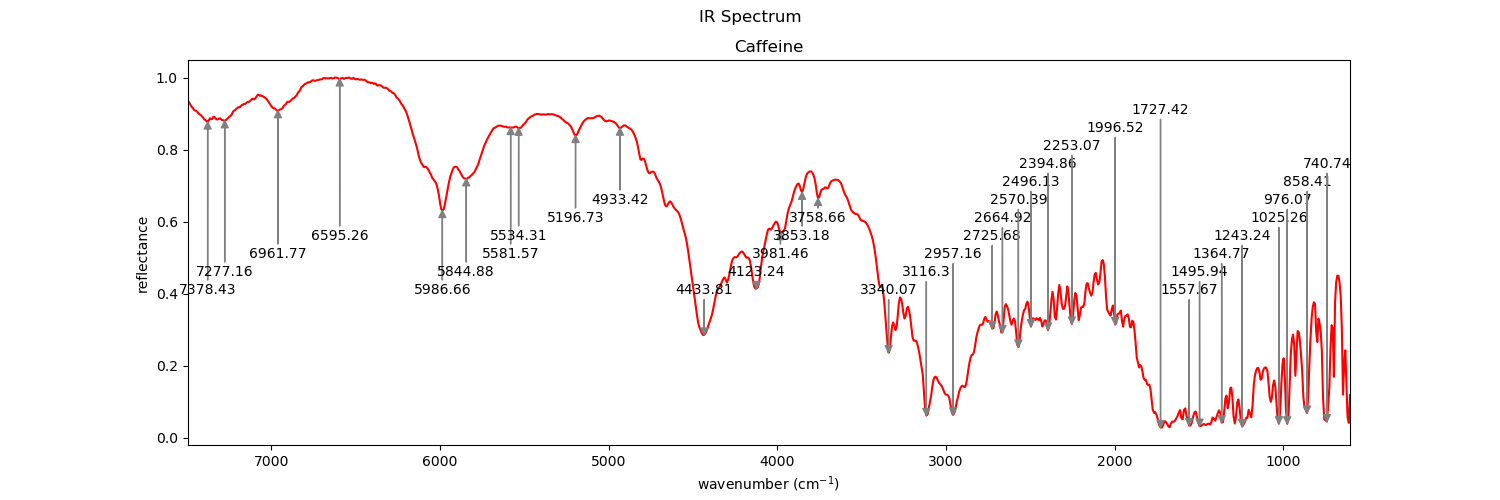
\includegraphics[width=\linewidth]{./task1-endresult}
\captionof{figure}{Spectrum of caffeine with marked absorption bands}
\label{fig:SpectrumCaffeine}
\end{minipage}

(or at least something that comes close to the shown picture.)

\subsection{About the source data}
On GRIPS you'll find the file \texttt{caffeine.jdx}. This file was downloaded as is from the public NIST chemical data base and can be found following the link \url{https://webbook.nist.gov/cgi/cbook.cgi?ID=C58082&Type=IR-SPEC&Index=1}. It contains an infrared reflection spectrum of caffeine in the \emph{JCAMP Chemical Spectroscopic Data Exchange Format}. This is a CSV based file format used by various software packages commonly used in chemistry. You can open and read it with a regular text editor.

As you can see, the file comprises of two blocks, representing two separate measurement sequences. Each block begins with comments which are marked by pound symbols  (\texttt{\#}) and end with the line \texttt{\#\#END=}. The comments contain meta information such as the date of measurement which we can ignore. The only exception is the line beginning with \texttt{\#\#TITLE=...}.

The real data are stored in tabular format. The columns are separated by whitespaces. In the first column you'll find the \emph{wave number} in $\text{cm}^{-1}$, \ie the values for the x-axis. The other columns hold the measured intensity, as observed by different detectors. We can ignore all but the first two columns.

Depending on the device used, the values may be \emph{normalized} to be between 0 and 1, or the file reports \emph{counts}, \ie an device-specific unit of measurement. For our plots we'll want to normalize all data, \ie we divide each value of a data set by its biggest value.

\subsection{Reading the Data into Memory}
Before you start develloping your class, first write some code that \enquote{only} reads the measurement data from the file and puts it into two Python \inPy{list}s \texttt{wavenumbers} and \texttt{intensities}. To do so, use the module \texttt{csv}. Also test whether or not you can create a plot. It should look something like this:

\begin{center}
	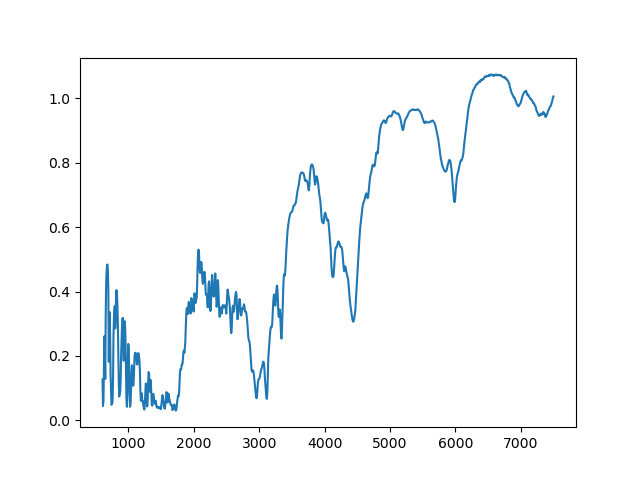
\includegraphics[width=.6\linewidth]{./spectrum-pre}
	\captionof{figure}{Spectrum of caffeine, not yet normalized, x-axis not yet inverted}
\end{center}

Once this works, expand your code such that the title of a measurement sequence is found in the file and stored in a variable. That means, find the line beginning with  \texttt{\#\#TITLE=} and store the end of this line.

\subsection{Attributes, First Methods}
Begin now designing your class \texttt{SpectrumPlot}. Answer to yourself whether you need any class attributes and if so, which ones. Also, identify the instance attributes you'll need. Have a look at the code you've already written for this analysis.

An additional instance attribute should be the \inPy{bool ready_to_plot} which we set to \inPy{False} be default. It indicates if all the necessary calls to the MatPlotLib have been made previously, \ie if the plot has been prepared in memory and can be shown right away.

Write a method \inPy{loadFile(self, filename)}. This method should deal with loading the file into memory. Your method \inPy{__init__} should call this \texttt{loadFile}. Make sure that \texttt{loadFile} also resets \inPy{ready_to_plot} to \inPy{False}. \emph{Optionally}, make it so that it is possible to create an instance of \texttt{SpectrumPlot} without loading a file.

\emph{Background}:\\
You \emph{could} write your code such that \inPy{__init__} on its own deals with loading the file. However, it makes codes easier to maintain if one method only performs one task itself. \emph{Preparation of the instance attributes} is one task; \emph{load a file} is another thought.

Now go on to write the methods \texttt{preparePlot} and \texttt{show}. If \inPy{ready_to_plot == False}, your method \texttt{show} should first call \texttt{preparePlot}. In either case, the next thing that \texttt{show} does is \texttt{self.fig.show()}. The method \texttt{preparePlot} should contain all the relevant calls to functions in the MatPlotLib to generate the plot object \emph{in memory}. In which method should we set \inPy{ready_to_plot = True}?

For now, ignore that we need to find and draw the minima of the spectrum. Do, however, respect the fact that the x-axis is in \emph{descending order}, \ie big wavenumbers are to the \emph{left}.

\emph{Background}:\\
Of course it would be easier to write only a single method \texttt{show} that prepares the plot and puts it on screen right away. However, as a user you might want to change some details of the plot and deviate from the default behaviour of your class. You might want to superimpose another plot of a different measurement sequence. If the plot was shown right away, this would lead to some unpleasant flickering.\\
In this exercise, we will not make use of this design feature; it still is good practice to write code such that it can be expanded easily.

\subsection{Finding Minima}
Now write a method \texttt{findMinima} that identifies the local minima of the plot.

\emph{Hint}:\\
You'll need to introduce at least one new instance attribute.

\emph{Attention}:\\
In practice, measurement data are always subject to \emph{noise} (small fluctuations in the measured data). As humans we might perceive a section of the plot as flat, but in reality there are tiny variations in the numerical value. As a consequence, there are \emph{tons} of \enquote{false} minima in the measured data. Can you think of a means to detect or suppress such false minima?

\emph{Note}:\\
Your method certainly needs not to be perfect. If you make it such that not every bit of noise is detected as minimum, you've already \enquote{won the match}.

\subsection{Show the Minima}
Expand your method \texttt{preparePlot} such that the found minima are marked in the plot with an arrow and a caption, such as in figure \ref{fig:SpectrumCaffeine}. When should \texttt{findMinima} be called?

\emph{Hint}:\\
The MatPlotLib sometimes cannot handle vertical arrows. If you run into trouble drawing an arrow from \texttt{(x, y1)} to \texttt{(x, y2)}, try drawing one to \texttt{(x + 1, y2)} instead. It looks essentially the same (given big enough values for \texttt{x}) and the MatPlotLib can handle it without problems.

\subsection{Test Robustness}
Now use your Class \texttt{SpectrumPlot} to also load the file \texttt{ethanol.jdx}\footnote{also found in the NIST data base. See \url{https://webbook.nist.gov/cgi/cbook.cgi?ID=C64175&Mask=80}}. In solution you'll find tomorrow on GRIPS, the following lines:
\begin{minted}{python3}
ethanol = SpectrumPlot("ethanol.jdx")
ethanol.supTitle = "IR Gas Phase Spectrum"
ethanol.linetype = "b:"
ethanol.ylabel = "transmittivity"
ethanol.show()
\end{minted}

will cause the following output:

\begin{minipage}{\linewidth}
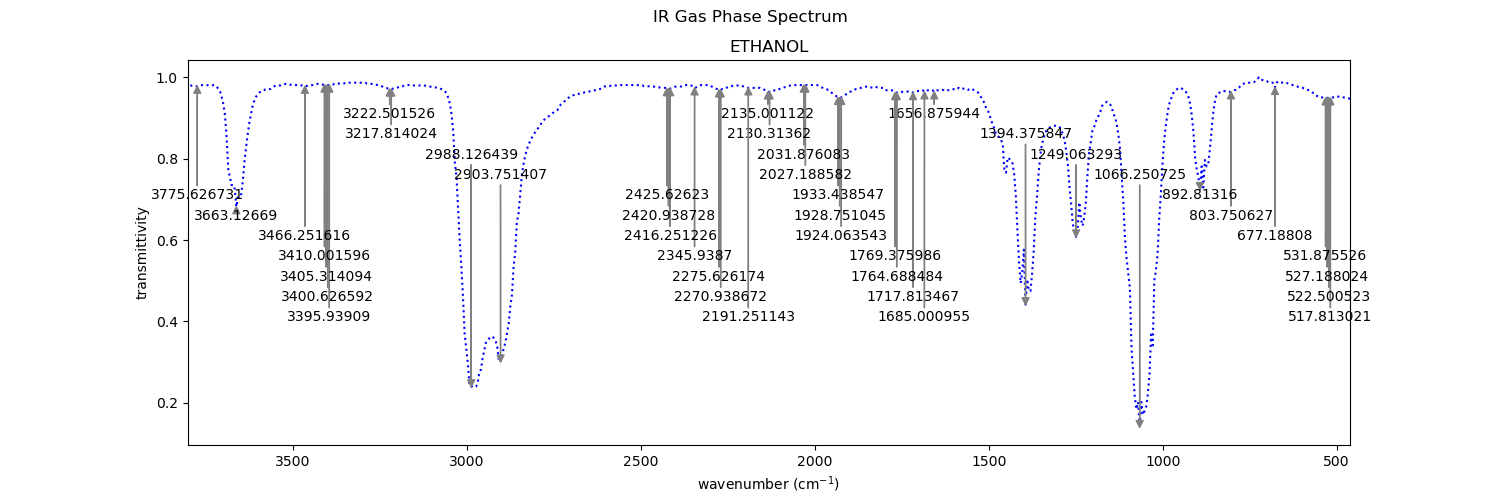
\includegraphics[width=\linewidth]{./task1-endresult-ethanol}
\captionof{figure}{Spectrum of ethanloe with marked absorption bands}
\end{minipage}


\section{Heartbeat (2\;P)}
Create a plot like in figure \ref{fig:hearts}:\\
\begin{minipage}{\linewidth}
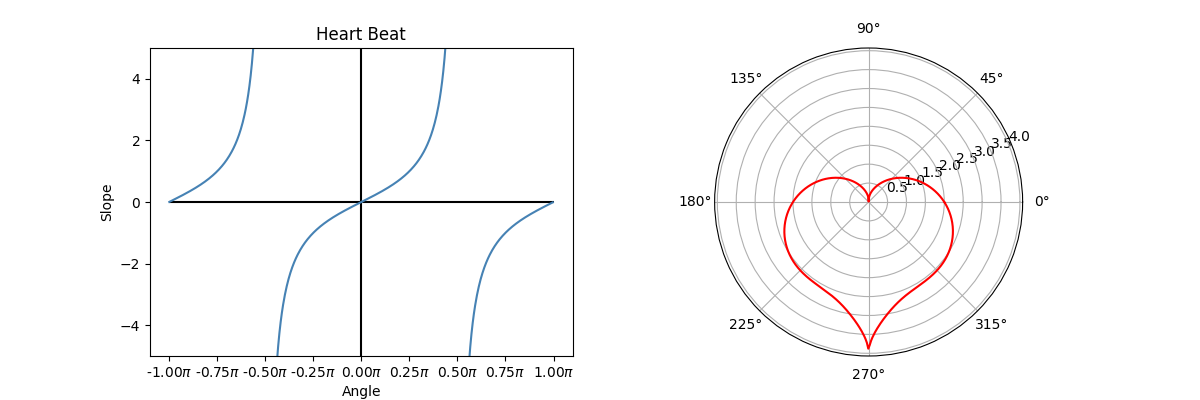
\includegraphics[width=\linewidth]{./task2}
\captionof{figure}{Heart Themed Functions}
\label{fig:hearts}
\end{minipage}

For the heartbeat, use the \texttt{math.tan} function. For the heart, use this equation\footnote{Source: \url{https://pavpanchekha.com/blog/heart-polar-coordinates.html}}
\begin{minted}{python3}
heart = lambda t : (math.sin(t) * math.sqrt( abs(math.cos(t)) )) / \
                   (math.sin(t) + 7/5) - 2 * math.sin(t) + 2
\end{minted}

To generate horizontal and vertical lines, you can use the commands \texttt{plt.hlines} and \texttt{plt.vlines}. Look up the details online.

Note that the poles should not be connected (no vertical lines at $\pm \frac{\pi}{2}$). Also make sure that the ticks are placed at quarter-integer multiples of pi. To insert the $\pi$ symbol, use the \LaTeX~ symbol \texttt{\$pi\$}.

\section{Evolution of the Sun (1\;P)}
On GRIPS you'll find the file \texttt{solar-evolution.py} which generates some data. With this, create the plot in figure \ref{fig:solar} (or something that comes close to that):
\begin{center}
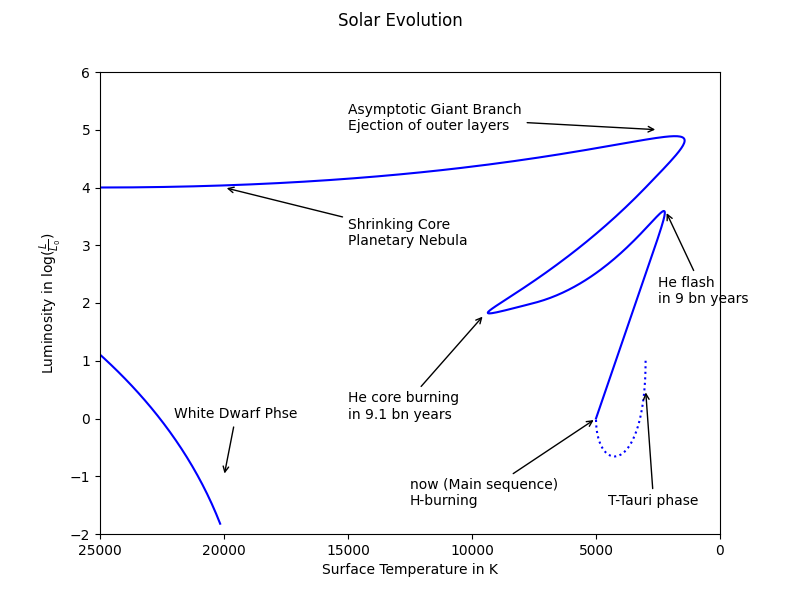
\includegraphics[width=.8\linewidth]{./task3}
\captionof{figure}{Transmission probabilities in a boson sampling device}
\label{fig:solar}
\end{center}

\emph{Hints}:\\
You don't need to understand what the functions \texttt{bezier} and \texttt{get\_smooth\_curve} do in detail. (See below if you would like to, anyway). All you'll need for this problem are the \inPy{tuple}s \texttt{dotted\_X}, \texttt{dotted\_Y}, \texttt{solid\_X} and \texttt{solid\_Y} which contain the x- and y-coordinates of the dotted and solid line in the plot, as the name suggests.

For the y-axis, use the label \inPy{r"log($\frac{L}{L_0}$)"}.

\emph{Background: what the plot shows}:\\
This is a (terribly inaccurate) prediction of the future of our sun. The dotted line represents the time as a proto star where the sun was not yet dense enough to maintain nuclear fusion. From that state the sun follows the track laid out by the plot, \ie it will become hotter/colder and brighter/dimmer over time, depending on which physical processes are going on inside the sun. The track is not followed at constant speed; most of the sun's lifetime (ca. 9 billion of the ca. 12 billion years) is spent in the \emph{main sequence phase} in which we are right now. Swelling to a red giant takes \enquote{a mere} 3 billion years before the onset of Helium fusion (\emph{He flash}) marks the transition in a new phase of the sun's life. After a \enquote{brief} (100 million year long) phase of fusing Helium in its core the sun swells a second time to a red supergiant which, over the course of some five million years, blasts out most of its mass as stellar wind. The remaining stellar core contracts over a period of some 100 000 years into a white dwarf, which slowly fades to oblivion over the course of some ten billion years. (In the white dwarf phase, nuclear fusion no longer takes place; hence, this phase is not considered part of the \enquote{lifetime} of a star.)

(Hey, I spent an entire semester abroad studying this stuff, something useful had to come from this, right?)

\emph{Background: Bezier curves}:\\
The code in \texttt{solar-evolution.py} is a (crude) implementation of the concept of Bezier curves. Bezier curves are smooth connections between two points that don't take the direct path but rather approach some intermediate point before going back to the original destination. You can watch this super-easy-to-understand video here for the mathematical background on them: \url{https://youtu.be/aVwxzDHniEw}\\
Bezier curves are used a lot in computer graphics, because they are easy to implement, cheap in terms of runtime and have convenient mathematical properties that can be exploited for a lot of algorithms.\\
I stitched together some Bezier curves to approximate the evolution of the sun, given little more than some boundary data points taken from my scripts (the numbers you used to define \texttt{solid\_through} and \texttt{dotted\_through}). As mentioned above, the result is not super accurate but qualitatively reflects the evolution our source of life will take in the long run.


\section{Transmission Probabilities (3\;P)}
On GRIPS you'll find the file \texttt{transition-probabilties.txt}. It is the result of a simulation I've written in for my physics master thesis. From this, create the plot in figure \ref{fig:transmission}.

\begin{center}
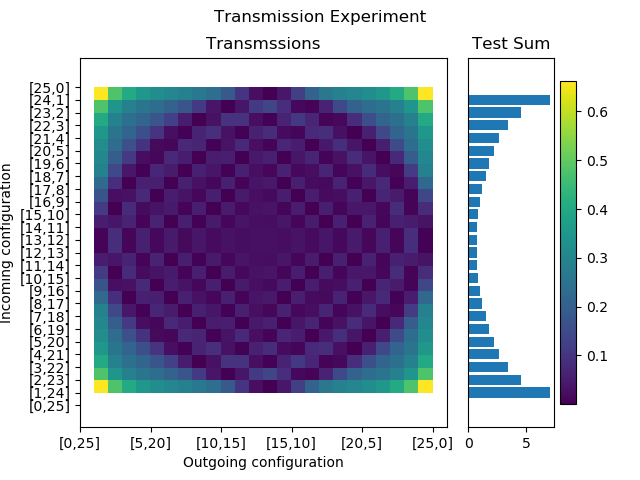
\includegraphics[width=.8\linewidth]{./task4}
\captionof{figure}{Transmission probabilities in a boson sampling device}
\label{fig:transmission}
\end{center}

\emph{Instructions:}\\
The file \texttt{transition-probabilties.txt} is based on the CSV format. The separator character is the tabulator (\inPy{"\t"}). You'll find two data blocks. The first of which describes the \enquote{coloured area}, while the second block is used in the bar chart. Each data block begins with a number of header lines that you can ignore. You'll recognize the data blocks by the first line which always begins with \texttt{incoming}. This first line (\ie the one beginning with \texttt{incoming}) also contains the column heads. The lines thereafter hold the column heads (\eg \texttt{[12,13]}) in the first column. The other columns hold the simulation data. A data block ends with a blank line.

You'll also notice that there are several cells where the result was \texttt{nan}, which stands for \emph{not a number}. In computing, operations that are aborted due to mathemtatical errors (such as computing $\sqrt{-1}$) often give this error value \texttt{nan}. Python and the MatPlotLib can handle this just fine: \inPy{float("nan")} yields the \enquote{numerical value} \texttt{nan}; when trying to plot the numerical value \texttt{nan}, the MatPlotLib simply draws nothing.

Read the file line by line (with a \texttt{csv reader}) and check, whether it begins with \texttt{incoming}. If so, you've reached a data block. Convert all data with \inPy{float(columnValue)} in numerical values and store them in a 2D list. After the first blank line, skip everything up to the first line starting with \texttt{incoming}. Then again, read the subsequent values to get a 1D list.
\end{document}
